\documentclass{article}
\usepackage[UTF8]{ctex}
\usepackage{amsmath,mathtools,geometry,cases,enumitem,amsfonts,amssymb,graphicx,float,tikz,fancyhdr,caption}
\usetikzlibrary{positioning,shapes.geometric}
\pagenumbering{arabic}
\pagestyle{fancy}
\fancyhead[L]{励志AQ班}
\fancyhead[R]{每日一题合集}
\fancyfoot[C]{\thepage}
\geometry{a4paper,scale=0.7}
\title{\vspace*{-1em}{\huge\textbf{每日一题合集}}}
\author{\kaishu李衡岳、\textbf{程昊一}、门宇翎、李东宸、王一丁、李政毅}
\date{}

\begin{document}
\maketitle

{\centering\tableofcontents}
\newpage\section{关于选题人的说明}
\textbf{1.}每日一题(($3n-2$).1)与(($3n-2$).2)由李衡岳、程昊一选题($n\in\mathbb{N}_+, n\le3$), 每日一题(($3n-2$).1)与(($3n-2$).2)至少由门宇翎选题($n\in\mathbb{N}_+, n>3$);
\par\hspace*{1em}每日一题(($3n-1$).1)与(($3n-1$).2)由门宇翎、李东宸选题($n\in\mathbb{N}_+, n\le3$), 每日一题(($3n-1$).1)与(($3n-1$).2)至少由李东宸选题($n\in\mathbb{N}_+, n>3$);
\par\hspace*{1em}每日一题(($3n$).1)与(($3n$).2)由王一丁、李政毅选题($n\in\mathbb{N_+}, n\le 2$), 每日一题(($3n$).1)与(($3n$).2)至少由李政毅选题($n\in\mathbb{N_+}, n>2$).
\par\hspace*{1em}所有的每日一题文档(包括此文档)及答案均为程昊一制作.\\
\par\textbf{2.}从每日一题(4.1)开始,记录每道题的供题者.
\newpage\section{七年级第一学期}

{\centering\subsection*{每日一题(1.1)}}
\addcontentsline{toc}{subsection}{每日一题(1.1)}
\par\textbf{1.}有一副27张的多米诺骨牌,现将其放入4$\times$14的方格中,每张骨牌有两个方格的大小,并将此方格的右上角与左下角去掉.证明:在不损伤骨牌的情况下,无法将54个方格完全铺满.\\
\begin{figure}[H]%1.1.1
	\centering
	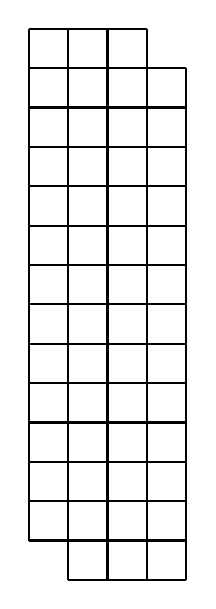
\begin{tikzpicture}
		\foreach \x in{0.5,1,1.5,2,2.5,3,3.5,4,4.5,5,5.5,6,6.5}{
			\draw[thick](0,\x)--(2,\x);
		}		
		\draw[thick](0.5,0)--(2,0);
		\draw[thick](0,7)--(1.5,7);
		\draw[thick](0,0.5)--(0,7);
		\draw[thick](2,0)--(2,6.5);
		\foreach \x in{0.5,1,1.5}
		\draw[thick](\x,0)--(\x,7);
	\end{tikzpicture}
	\caption{每日一题(1.1):第一题图}
\end{figure}
\par\textbf{2.}(1)证明:$\sqrt{2}$不是有理数.
\par\hspace*{3.5mm}(2)证明:当$n$不为完全平方数时,$\sqrt{n}$是否为无理数?\\

{\centering\subsection*{每日一题(1.2)}}
\addcontentsline{toc}{subsection}{每日一题(1.2)}
\par\textbf{1.}如图,求$\angle A+\angle B+\angle C+\angle D+\angle E+\angle F+\angle G$的值.
\begin{figure}[H]%1.2.1
	\centering
	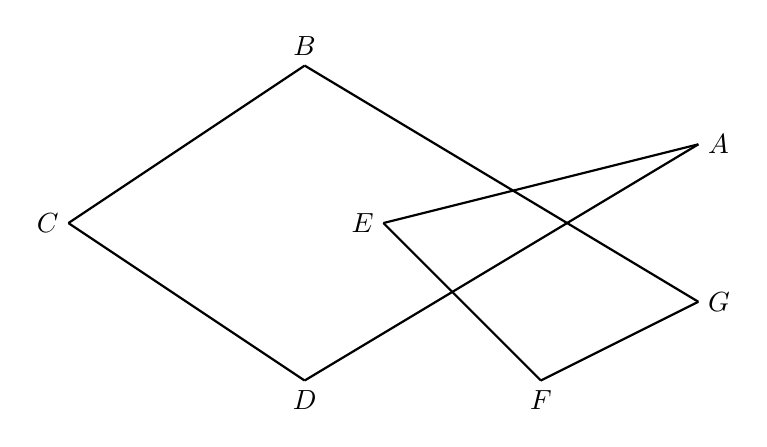
\begin{tikzpicture}
		\node at (5,1) [anchor=west]{$A$};
		\node at (0,2) [anchor=south]{$B$};
		\node at (-3,0) [anchor=east]{$C$};
		\node at (0,-2) [anchor=north]{$D$};
		\node at (1,0) [anchor=east]{$E$};
		\node at (3,-2) [anchor=north]{$F$};
		\node at (5,-1) [anchor=west]{$G$};
		\draw[thick](5,1)--(0,-2);
		\draw[thick](0,-2)--(-3,0);
		\draw[thick](-3,0)--(0,2);
		\draw[thick](0,2)--(5,-1);
		\draw[thick](5,-1)--(3,-2);
		\draw[thick](3,-2)--(1,0);
		\draw[thick](1,0)--(5,1);	
	\end{tikzpicture}
	\caption{每日一题(1.2):第一题图}
\end{figure}
\par\textbf{2.}用4个大小相等的方格可以组成7种图案(不计旋转),如图所示.证明:不能用他们密铺一个4行7列的网格.
\begin{figure}[H]%1.2.2
	\centering
	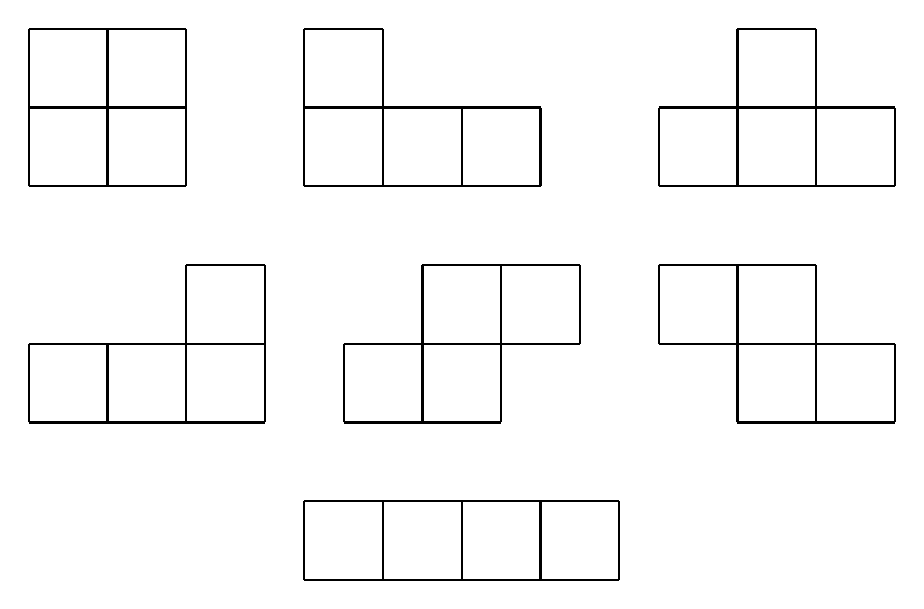
\begin{tikzpicture}
		\foreach \x in{0,1,2}
		\draw[thick](\x,0)--(\x,2);
		\foreach \y in{0,1,2}
		\draw[thick](0,\y)--(2,\y);
		\foreach \x in{5.5,6.5,8,11}
		\draw[thick](\x,0)--(\x,1);
		\foreach \x in{3.5,4.5,9,10}
		\draw[thick](\x,0)--(\x,2);
		\draw[thick](3.5,2)--(4.5,2);
		\draw[thick](9,2)--(10,2);
		\draw[thick](3.5,1)--(6.5,1);
		\draw[thick](8,1)--(11,1);
		\draw[thick](3.5,0)--(6.5,0);
		\draw[thick](8,0)--(11,0);
		\draw[thick](2,-1)--(3,-1);
		\draw[thick](5,-1)--(7,-1);
		\draw[thick](8,-1)--(10,-1);
		\foreach \x in{0,4,8}
		\draw[thick](\x,-2)--(\x+3,-2);
		\draw[thick](0,-3)--(3,-3);
		\draw[thick](4,-3)--(6,-3);
		\draw[thick](9,-3)--(11,-3);
		\foreach \x in{2,3,5,6,7,8,9,10}
		\draw[thick](\x,-2)--(\x,-1);
		\foreach \x in{0,1,2,3,4,5,6,9,10,11}
		\draw[thick](\x,-3)--(\x,-2);
		\draw[thick](3.5,-4)--(7.5,-4);
		\draw[thick](3.5,-5)--(7.5,-5);
		\foreach \x in{3.5,4.5,5.5,6.5,7.5}
		\draw[thick](\x,-4)--(\x,-5);	
	\end{tikzpicture}
	\caption{每日一题(1.2):第二题图}
\end{figure}

{\centering\subsection*{每日一题(2.1)}}
\addcontentsline{toc}{subsection}{每日一题(2.1)}
\par\textbf{1.}在实数范围内解方程:
\[\sqrt{x}+\sqrt{y-1}+\sqrt{z-2}=\frac{1}{2}(x+y+z)\]
\par\textbf{2.}已知$a,b,c$为一个三角形的三边长,且满足
\[a^2+b^2+c^2+338=10a+24b+26c\]
试判断此三角形的形状.\\

{\centering\subsection*{每日一题(2.2)}}
\addcontentsline{toc}{subsection}{每日一题(2.2)}
\par\textbf{1.}若方程组
\[\begin{cases}
	a_1x+b_1y=c_1\\a_2x+b_2y=c_2\\
\end{cases}\]
的解为$(x,y)=(3,4)$,求方程组
\[\begin{cases}
	3a_1x+2b_1y=5c_1\\3a_2x+2b_2y=5c_2\\
\end{cases}\]
的解.\\\quad\\
\par\textbf{2.}已知关于$x,y$的方程组
\[\begin{cases}
	2x-ay=6\\4x+y=7\\
\end{cases}\]
的解为整数,$a$为正整数,求$a$的值.\\

{\centering\subsection*{每日一题(3.1)}}
\addcontentsline{toc}{subsection}{每日一题(3.1)}
\par\textbf{1.}已知$a,b,c$为实数,且$a-b=4,ab+c^2+4=0$,求$a+b$的值.\\
\par\textbf{2.}已知$a+\dfrac{1}{a}=5$,求$\dfrac{a^4+a^2+1}{a^2}$的值.\\

{\centering\subsection*{每日一题(3.2)}}
\addcontentsline{toc}{subsection}{每日一题(3.2)}
\par\textbf{1.}求所有这样的素数,它加上10或14后,仍为素数.\\
\par\textbf{2.}证明:从1至100(包括1和100)中任选51个数,其中必有两个数互素.
\par 思考:题中的“51”还可以更小吗?\\
\par\textbf{3.}将平面上所有的点都染成红、蓝两色,证明:存在一条长为1的线段,它的端点同色.
\par 思考:若平面不为全红或全蓝,是否总存在一条长为1的线段,其端点异色?若将平面染成三种颜色,是否仍然存在长为1的端点同色的线段?\\

{\centering\subsection*{每日一题(4.1)}}
\addcontentsline{toc}{subsection}{每日一题(4.1)}
\par\textbf{1.}用纯数学的方法证明圆锥的体积公式
\[V=\frac{1}{3}\pi r^2h\]
{\CJKfamily{kai}(李衡岳供题)}\\
\par\textbf{2.}求所有的整数$x,y$,使得$x^2+xy+y^2=1$.\\
{\CJKfamily{kai}(程昊一供题)}\\

{\centering\subsection*{每日一题(4.2)}}
\addcontentsline{toc}{subsection}{每日一题(4.2)}
\par\textbf{1.}用含$n$的代数式表示$1^4+2^4+\dots+n^4$,其中$n$为正整数.\\
{\CJKfamily{kai}(程昊一供题)}\\
\par\textbf{2.}平面上有25个点,任意三点之中必然存在两个点,它们的距离小于1.证明:必然能找到13个点,它们位于半径为1的圆中.\\
{\CJKfamily{kai}(程昊一供题)}\\

{\centering\subsection*{每日一题(5.1)}}
\addcontentsline{toc}{subsection}{每日一题(5.1)}
\par\textbf{1.}若$n$为正整数,且$2^n-1$为素数,证明:$n$也为素数.\\
{\CJKfamily{kai}(门宇翎供题)}\\
\par\textbf{2.}如图,两个同心圆构成的圆环被均匀分割成7份,联通中间的校园共8个区域.若要给这8个区域着色,至少要用几种颜色,才能使相邻区域染不同的颜色?\\
\begin{figure}[H]%5.1.2
	\centering
	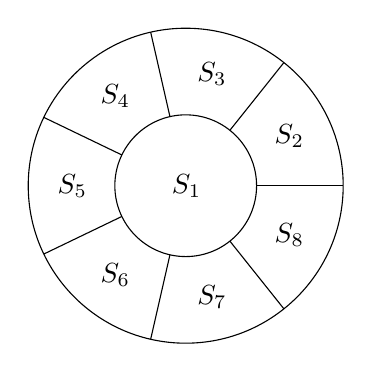
\begin{tikzpicture}
		\draw (0,0) circle(0.9);
		\node at (-0.3,0) [right]{$S_1$};
		\draw (0,0) circle(2);
		\foreach \x in {0,1,2,3,4,5,6}
		\draw [rotate={51.42857 * \x}] (0.9,0)--(2,0);
		\node at (1.0064,0.6291)[right]{$S_2$};
		\node at (0.0227,1.4136)[right]{$S_3$};
		\node at (-1.2041,1.1336)[right]{$S_4$};
		\node at (-1.75,0)[right]{$S_5$};
		\node at (-1.2041,-1.1337)[right]{$S_6$};
		\node at (0.0227,-1.4136)[right]{$S_7$};
		\node at (1.0064,-0.6291)[right]{$S_8$};
		
	\end{tikzpicture}
	\caption{每日一题(5.1):第二题图}
\end{figure}
{\CJKfamily{kai}(李东宸供题)}\\

{\centering\subsection*{每日一题(5.2)}}
\addcontentsline{toc}{subsection}{每日一题(5.2)}
\par\textbf{1.}若$n$为正整数,$2^n+1$为素数,求证:$n$为2的幂,即存在自然数$k$,使得$n=2^k$.\\
{\CJKfamily{kai}(门宇翎供题)}\\
\par\textbf{2.}将正七边形的七个顶点染红、蓝两色,证明必存在一个顶点均同色的等腰三角形.\\
{\CJKfamily{kai}(李东宸供题)}\\

{\centering\subsection*{每日一题(6.1)}}
\addcontentsline{toc}{subsection}{每日一题(6.1)}
\par\textbf{1.}求满足$ 5x-2[x]=-8 $的所有$ x $,其中$ [x] $表示不超过$ x $的最大整数.\\
{\CJKfamily{kai}(王一丁供题)}\\
\par\textbf{2.}在2003$ \times $2003的小方格中,随意写上1或-1,然后将每一列中的乘积写在其下方,将每一行中的乘积写在其右边,这样得到4006个数,证明:这4006个数的和不等于0.\\
{\CJKfamily{kai}(李政毅供题)}\\

{\centering\subsection*{每日一题(6.2)}}
\addcontentsline{toc}{subsection}{每日一题(6.2)}
\par\textbf{1.}证明$ 3^{2012}+4^{2013} $是5的倍数.\\
{\CJKfamily{kai}(王一丁供题)}\\
\par\textbf{2.}证明:不存在整数$ x,y $,使得$ x^2+y^2=2015 $.\\
{\CJKfamily{kai}(李政毅供题)}
\newpage\section{七年级第二学期}

{\centering\subsection*{每日一题(7.1)}}
\addcontentsline{toc}{subsection}{每日一题(7.1)}
\par\textbf{1.}我们定义:如果$a$($a>0$且$a\neq 1$)的$b$次幂等于$N$,那么 $b$称为以$a$为底$N$的对数,记作
\[\log_aN=b.\]
证明:若$a,b>0,a,b\neq 1$,则
\begin{itemize}
	\item[(1)]$\log_ax+\log_ay=\log_axy$\quad$(x,y>0)$;
	\item[(2)]$\log_ax^b=b\log_ax$\quad$(x>0)$;
	\item[(3)]$\log_ax=\dfrac{\log_bx}{\log_ba}$\quad$(x>0)$;
	\item[(4)]$\log_{a^x}b^y=\dfrac{y}{x}\log_ab$\quad$(x\neq 0)$.
\end{itemize}
{\CJKfamily{kai}(程昊一供题)}\\
\par\textbf{2.}有$n$个人,每个人的生日是完全随机且互不相关的.当$n$不小于多少时,存在两个生日相同的人的概率不小于$\dfrac{1}{2}$(假设一年有365天)?\\
{\CJKfamily{kai}(李衡岳供题)}\\

{\centering\subsection*{每日一题(7.2)}}
\addcontentsline{toc}{subsection}{每日一题(7.2)}
\textbf{1.}求所有的整数$x,y$,满足方程
\[(x^2-y^2)^2=16y+1.\]
{\CJKfamily{kai}(程昊一供题)}\\
\par\textbf{2.}我们假设有一个村庄,村庄里有很多户人家.每一户人都有一条狗,可能是正常的狗,也可能是疯狗.如果一个人发现自己的狗是疯狗,那么他会在当天晚上把自己的狗击毙.每一个人只可以判断其他人的狗是否为疯狗,每两个人之间也不能互相交流.一天,一位游客向全部的人宣布:“村庄里有疯狗!”当天晚上,没有人击毙自己的狗;第二天亦是如此;第三天有人击毙了自己的狗.问:村庄里有几条疯狗?\\
{\CJKfamily{kai}(李衡岳供题)}\\

{\centering\subsection*{每日一题(8.1)}}
\addcontentsline{toc}{subsection}{每日一题(8.1)}
\textbf{1.}阅读材料:
{\kaishu
	\par 对于形如$\sqrt{m\pm\sqrt{n}}$的复合二次根式, 我们可以采取以下的方式化简: \\
	(1)\quad 找到合适的$a$和$b$, 使得$a+b=m$, $4ab=n$.\\
	(2)\quad 将原式做变形:
	\begin{align*}
		\sqrt{m\pm\sqrt{n}}&=\sqrt{a+b\pm\sqrt{4ab}}\\
		&=\sqrt{\left(\sqrt{a}\right)^2+\left(\sqrt{b}\right)^2\pm2\cdot\sqrt{a}\cdot\sqrt{b}}\\
		&=\sqrt{\left(\sqrt{a}\pm\sqrt{b}\right)^2}\\
		&=\left|\sqrt{a}\pm\sqrt{b}\right|.
	\end{align*}
	(3)\quad 即得答案:$\sqrt{m\pm\sqrt{n}}=\left|\sqrt{a}\pm\sqrt{b}\right|$.
}
\par 化简: 
\begin{itemize}
	\item[(1)]$\sqrt{5+2\sqrt{6}}$ ; 
	\item[(2)]$\sqrt{7-2\sqrt{12}}$ . 
\end{itemize}
{\kaishu (李东宸供题)}\\
\par \textbf{2.}证明: 若$a$, $b$是大于1的正整数, 则 $a^4+4b^4$是合数.\\
{\kaishu (门宇翎供题)} 

{\centering\subsection*{每日一题(8.2)}}
\addcontentsline{toc}{subsection}{每日一题(8.2)}
\textbf{1.}若$x$, $y$均为实数, 且满足方程
\[x^2+y^2+4x-6y+13=0,\]
求$x+2y$的值.\\
{\kaishu (李东宸供题)}\\

\par\textbf{2.}某会议共有30名议员, 每两个人之间互相的关系为朋友或政敌. 每个人都有且仅有6个政敌. 每3个人组成一个委员会. 若一个委员会内的三个人的关系均为朋友或政敌, 则称这个委员会为“好委员会”. 求“好委员会”的数量. \\
{\kaishu (门宇翎供题)}

{\centering\subsection*{每日一题(9.1)}}
\addcontentsline{toc}{subsection}{每日一题(9.1)}
\textbf{1. }已知:
\[\left(a^2+b^2+c^2\right)\left(x^2+y^2+z^2\right)=(ax+by+cz)^2\quad(a,b,c\neq0),\]
求证: $\dfrac{x}{a}=\dfrac{y}{b}=\dfrac{z}{c}$.\\\par
\textbf{2. }已知$a-b=4$, $ab+c^2+4=0$, 求$a+b$的值.\\

{\centering\subsection*{每日一题(9.2)}}
\addcontentsline{toc}{subsection}{每日一题(9.2)}
\textbf{1. }若$m^2=n+2, n^2=m+2$ $(m\neq n)$, 求$m^3-2mn+n^3$的值.\\\par
\textbf{2. }已知$a+b-c=9, a^2+b^2+c^2=27$, 求$a^{2009}+b^{2009}+c^{2009}$的值.\\

{\centering\subsection*{每日一题(10.1)}}
\addcontentsline{toc}{subsection}{每日一题(10.1)}
\textbf{1. }若实数$x$, $y$, $z$满足
\[x+y=4, |z+1|=xy+2y-9,\]
求$x+2y+3z$的值.\\\par
\textbf{2. }若$n$为整数, 证明: $n^2+n+1$不是完全平方数. \\

{\centering\subsection*{每日一题(10.2)}}
\addcontentsline{toc}{subsection}{每日一题(10.2)}
\textbf{1. }已知$x$, $y$, $z$为实数, 且满足
\[x+2y-5z=3, x-2y-z=-5,\]
求$x^2+y^2+z^2$的最小值.\\
\rightline{\kaishu (门宇翎供题)}\\\par
\textbf{2. }因式分解:
\[\left(x^2+2y^2\right)^4+64y^8.\]
\rightline{\kaishu (程昊一命题)}\\

{\centering\subsection*{每日一题(11.1)}}
\addcontentsline{toc}{subsection}{每日一题(11.1)}
\textbf{1. }已知$a$, $b$, $c$互不相等, 且满足
\[\frac{a+b}{a-b}=\frac{b+c}{2(b-c)}=\frac{c+a}{3(c-a)},\]
求证:
\[8a+9b+5c=0.\]\\
\rightline{\kaishu (李东宸供题)}\\\par
\textbf{2. }高斯函数$[x]$, 也称取整函数, 即$[x]$表示不超过$x$的最大整数. 则下面的命题中: 
\begin{enumerate}[noitemsep,label={(\arabic*)}]
	\item $[x]+[-x]=0$;
	\item 当$-1\le x<1$时, $[x+1]+[-x+1]$的值为$0$, $1$, $2$;
	\item $[x]+[y]=[x+y]$;
	\item 若$x\neq 1$, 则$[x]\cdot\left[\dfrac{1}{x}\right]=0$;
\end{enumerate}
哪些是正确的? 哪些是不正确的?\\
\rightline{\kaishu (李东宸供题, 程昊一改编)}

{\centering\subsection*{每日一题(11.2)}}
\addcontentsline{toc}{subsection}{每日一题(11.2)}
\textbf{1. }若$a$, $b$满足
\[3a^2+5|b|=7, s=2a^2-3|b|,\]
求$s$的取值范围.\\\par
\textbf{2. }运行程序如图所示, 规定: 从“输入一个值$x$”到“结果是否$>95$”为一次程序操作. 
如果程序运行了3次后停止, 求$x$的取值范围.
\begin{figure}[htbp]%11.2.2
	\centering
	\begin{tikzpicture}[node distance=10pt]
		\node [draw,rounded corners]                    (start)  {开始};
		\node [draw,below=of start]                     (input)  {输入};
		\node [draw,below=of input]                     (x)      {$x$};
		\node [draw,below=of x]                         (times2) {$\times2$};
		\node [draw,below=of times2]                    (+1)     {$+1$};
		\node [draw,diamond,aspect=2,below=of +1]       (>95)    {$>95$?};
		\node [draw,right=20pt of >95]                  (no)     {返回};
		\node [draw,rounded corners,below=15pt of >95]  (end)    {结束};
		
		\draw [->] (start)--(input);
		\draw [->] (input)--(x);
		\draw [->] (x)--(times2);
		\draw [->] (times2)--(+1);
		\draw [->] (+1)--(>95);
		\draw [->] (>95)-- node[left]{是} (end);
		\draw [->] (>95)-- node[above]{否} (no);
		\draw [->] (no)-- (no|-x) -> (x);
	\end{tikzpicture}
	\caption*{\kaishu 第二题图}
\end{figure}
\end{document}
